% !TeX encoding = UTF-8
\documentclass[12pt]{article}
\usepackage[spanish]{babel}
\usepackage[utf8]{inputenc}
\usepackage{graphicx} % Required for inserting images
\usepackage{geometry}
\usepackage{adjustbox}
\usepackage[most]{tcolorbox}
\usepackage[hidelinks]{hyperref}
\usepackage{parskip}
\usepackage{float}
\usepackage{blindtext}
\usepackage{csquotes}
\usepackage{svg}
\usepackage[
    backend=biber,
    style=numeric,
    sorting=none
]{biblatex}
\usepackage{microtype}
\usepackage{listings}
\usepackage{listingsutf8}
\lstdefinestyle{ascii-tree}{
	escapeinside={&*}{*&},
	literate=
	{├}{{\smash{\raisebox{-1ex}{\rule{1pt}{\baselineskip}}}\raisebox{0.5ex}{\rule{1ex}{1pt}}}}1 
	{─}{{\raisebox{0.5ex}{\rule{1.5ex}{1pt}}}}1 
	{└}{{\smash{\raisebox{-1ex}{\rule{1pt}{\baselineskip}}}}}1 % (O como lo tengas)
}
 \usepackage{dirtree}
 \usepackage{xspace}
\addbibresource{TFG.bib}

\title{Inteligencia Artificial On‑Premise para el análisis de IoCs con datos privados}
\author{Nicolás Pueyo Soria}
\date{Junio 2026}

\newcommand{\pipelines}{\textit{Pipelines}}
\newcommand{\OpenWebUI}{\textit{OpenWebUI}}
	
\setlength{\paperwidth}{21cm}          % Ancho de página
\setlength{\paperheight}{29,7cm}       % Alto de página
\setlength{\textwidth}{15.5cm}         % Ancho de zona con texto
\setlength{\textheight}{24.6cm}        % Ancho de zona con texto
\setlength{\topmargin}{-1.0cm}         % Margen superior
                                      
\setlength{\oddsidemargin}{0.46cm}     % Margen izquierdo 
\setlength{\evensidemargin}{0.46cm}    

\setcounter{secnumdepth}{4}
\setcounter{tocdepth}{4}
\newcommand{\subsubsubsection}[1]{\paragraph{#1}}

\makeatletter
\renewcommand\paragraph{\@startsection{paragraph}{4}{\z@}%
	{-3.25ex\@plus -1ex \@minus -.2ex}% Espaciado antes del título
	{1.5ex \@plus.2ex}% Espaciado después (un valor positivo fuerza el salto de línea)
	{\normalfont\normalsize\bfseries}} % Estilo de fuente (negrita, tamaño normal)
\makeatother



%%%%% DEFINICIÓN DE ESTILOS PARA LISTINGS
\definecolor{codegreen}{rgb}{0,0.6,0}
\definecolor{codegray}{rgb}{0.5,0.5,0.5}
\definecolor{codepurple}{rgb}{0.58,0,0.82}
\definecolor{backcolour}{rgb}{0.95,0.95,0.92}

\lstdefinestyle{mystyle}{
	backgroundcolor=\color{backcolour},   
	commentstyle=\color{codegreen},
	keywordstyle=\color{magenta},
	numberstyle=\tiny\color{codegray},
	stringstyle=\color{codepurple},
	basicstyle=\ttfamily\footnotesize,
	breakatwhitespace=false,         
	breaklines=true,                 
	captionpos=b,                    
	keepspaces=true,                 
	numbers=left,                    
	numbersep=5pt,                  
	showspaces=false,                
	showstringspaces=false,
	showtabs=false,                  
	tabsize=2
}

\lstset{style=mystyle}

\begin{document}

\pagenumbering{roman}
\renewcommand{\contentsname}{Índice}
\renewcommand{\labelitemi}{$\bullet$}
\renewcommand{\tablename}{Tabla}
\renewcommand{\lstlistingname}{Listado}
\renewcommand{\lstlistlistingname}{Índice de Listados}

\begin{titlepage}

\vspace*{-4mm}
\begin{figure}[!h]
  \centering
	
\includegraphics[width=69.62mm]{Imagenes/UnizarLogo}
\end{figure}

\vspace*{17mm}

\fontsize{28pt}{28pt}\selectfont
\begin{center}
\setlength{\fboxsep}{3.4mm}
\adjustbox{minipage=14.4cm,cfbox=blue,center}{\begin{center} Trabajo Fin de Grado
\end{center}}
\end{center}

\vspace{18.7mm}


\fontsize{20pt}{20pt}\selectfont
\begin{center}
Inteligencia Artificial On-Premise para el análisis de IoCs con datos privados
\end{center}

\vspace*{1cm} 
\baselineskip 36pt
\begin{center}
\fontsize{12pt}{12pt}\selectfont
\center{\rm  Autor}

\vspace*{3.65mm} 
\fontsize{18pt}{18pt}\selectfont
\center{Nicolás Pueyo Soria}
\vspace*{1.3cm}
\fontsize{12pt}{12pt}\selectfont
\center{\rm  Directores}
\vspace*{4.5mm}
\fontsize{14pt}{14pt}\selectfont
\center{Héctor Francia Molinero}
\center{Ricardo Julio Rodríguez Fernández}
\end{center}

\setcounter{footnote}{1}

\vspace*{16.45mm}
\fontsize{12pt}{12pt}\selectfont
\begin{center}
ESCUELA DE INGENIERÍA Y ARQUITECTURA\\
2026\\
\end{center}


\renewcommand{\thefootnote}{\arabic{footnote}}
\end{titlepage}


    
\newpage
%%%%%%%%%%%%%%%%%%%%%%%%%%%%%%%%%%%%%%%%%%
 %%%%% Agradecimientos
 %%%%%%%%%%%%%%%%%%%%%%%%%%%%%%%%%%%%%%%%%%
\section*{Agradecimientos}

\setcounter{page}{1}

\newpage
\begin{abstract}
    Aquí irá el abstract cuando acabe de escribir
\end{abstract}

\newpage
\renewcommand{\abstractname}{Abstract}
\begin{abstract}
    In English ig
\end{abstract}
\newpage
\tableofcontents

\newpage
\listoffigures
\listoftables
\lstlistoflistings

\newpage
\pagenumbering{arabic}

%%%%%%%%%%%%%%%%%%%%%%%%%%%%%%%%%%%%%%%%%%
%%%%%% Introducción
%%%%%%%%%%%%%%%%%%%%%%%%%%%%%%%%%%%%%%%%%%
\section{Introducción}
\subsection{Contexto y motivación}
En los últimos años, la adopción de tecnologías basadas en Inteligencia Artificial (IA) se ha consolidado como una práctica habitual en el entorno corporativo para optimizar procesos y mejorar la productividad de los empleados. En particular, los Modelos de Lenguaje de Gran Escala (LLM) han demostrado ser herramientas de utilidad para tareas como la síntesis de información y la redacción de informes técnicos. No obstante, este rápido despliegue tecnológico también introduce retos de seguridad significativos. La falta de formación específica en ciberseguridad de muchos usuarios puede dar lugar a malas prácticas en el manejo de la IA, como la exposición accidental de datos corporativos sensibles al enviarlos a APIs comerciales externas.

De forma paralela, la defensa frente a incidentes digitales se apoya cada vez más en la Ciberinteligencia de Amenazas (CTI, por sus siglas en inglés), la cual permite estructurar y correlacionar datos sobre potenciales ataques mediante herramientas de código abierto como OpenCTI. Sin embargo, la gestión diaria de estos repositorios de conocimiento sigue requiriendo una considerable inversión de tiempo por parte de los analistas para procesar e interpretar la información técnica de los nuevos Indicadores de Compromiso (IoC).

En este escenario, surge la oportunidad de integrar la IA generativa como un asistente para facilitar la labor de los analistas en la interpretación y análisis de CTI. Para llevar a cabo esta integración en un contexto empresarial de manera segura, es necesario descartar las soluciones basadas en la nube y optar por modelos locales y privados. De este modo, este proyecto propone el desarrollo de una herramienta desplegada en un servidor privado que, mediante modelos de lenguaje especializados ejecutados localmente, permita a los ingenieros de ciberseguridad consultar, comparar y contrastar la ciberinteligencia de la organización con nuevos indicadores en un tiempo razonable, garantizando la soberanía de los datos sensibles de la empresa.

El presente proyecto se ha desarrollado en el marco de colaboración con la división de Zaragoza de Inetum España S.A., multinacional especializada en consultoría tecnológica y provisión de servicios de TI. En Aragón, Inetum desempeña un papel relevante al gestionar las infraestructuras y los servicios informáticos de entidades públicas de gran envergadura, como la Diputación General de Aragón (DGA) y el Servicio de Salud Aragonés (SALUD). En este contexto empresarial, la infraestructura asignada para el despliegue de la solución consta de entornos de virtualización Linux (RedHat 10), sin entorno de escritorio, sobre hardware de centro de datos basados únicamente en capacidad de procesamiento (CPU) y memoria RAM, prescindiendo por completo de aceleración gráfica por GPU. Además, con el fin de garantizar la soberanía, la transparencia y la viabilidad de la arquitectura propuesta, el sistema se implementará de manera íntegra utilizando herramientas y soluciones de software de código abierto.

\subsection{Objetivos del proyecto}

El objetivo general de este proyecto es diseñar, implementar y evaluar una plataforma privada y local de asistencia conversacional orientada a la ingeniería de ciberseguridad, integrada con una plataforma de gestión de ciberinteligencia de amenazas (CTI). El sistema propuesto debe permitir la consulta interactiva y el análisis contextualizado de Indicadores de Compromiso (IoC) garantizando la soberanía de los datos sensibles y optimizando el rendimiento de modelos de lenguaje bajo restricciones estrictas de hardware basadas exclusivamente en procesamiento por CPU y memoria RAM.

Para alcanzar este fin, se proponen los siguientes objetivos específicos:

\begin{itemize}
    \item \textbf{Despliegue y configuración de un entorno local aislado:} Implementar una infraestructura privada que albergue un entorno de ejecución para modelos de lenguaje y una interfaz gráfica de usuario accesible para los analistas, operando de manera local y sin dependencias de servicios externos en la nube.
    \item \textbf{Desarrollo de un pipeline de recuperación semántica:} Diseñar un mecanismo de indexación, almacenamiento vectorial y recuperación semántica de datos que permita alimentar las consultas del asistente conversacional con la ciberinteligencia y el contexto histórico de la organización de forma precisa.
    \item \textbf{Integración y consulta bidireccional con sistemas de ciberinteligencia:} Establecer una conexión con la API de la plataforma de ciberinteligencia del cliente para permitir que el asistente interactúe con el grafo de conocimiento existente, traduciendo consultas en lenguaje natural a búsquedas estructuradas de observables y amenazas.
    \item \textbf{Evaluación comparativa de modelos de lenguaje especializados:} Evaluar el rendimiento, el nivel de detalle técnico, la tasa de alucinaciones y la precisión de múltiples modelos de lenguaje de diferentes escalas de parámetros en tareas complejas de correlación y análisis de indicadores.
\end{itemize}
\subsection{Estructura del documento}
El presente documento se estructura en diferentes secciones con subsecciones. En la segunda sección se explican los conocimientos teóricos previos a tener en cuenta sobre diferentes conceptos clave para entender el desarrollo del proyecto. En la tercera sección se detalla cuál es la arquitectura del proyecto, qué componentes se han utilizado, qué tecnologías se han usado para desarrollar o desplegar cada uno de estos componentes, así como qué organización tienen y cómo se despliegan físicamente cada uno, y finalmente explica el workflow general del sistema, es decir, cómo cumple cada componente su cometido. En la cuarta sección se detallan las pruebas que se han realizado al sistema, se recogen y presentan los resultados obtenidos y se realiza un análisis de los mismos. Finalmente, en la última sección, la quinta, se analiza todo el contexto y trabajo desarrollado para extraer unas conclusiones, y se reflexiona sobre qué otras funcionalidades se podrían añadir al proyecto en caso de continuar con el desarrollo.
\newpage
%%%%%%%%%%%%%%%%%%%%%%%%%%%%%%%%%%%%%%%%%%
%%%%%% Conceptos previos
%%%%%%%%%%%%%%%%%%%%%%%%%%%%%%%%%%%%%%%%%%
\section{Conceptos previos}
\subsection{IR e IoCs}

En el ámbito de la ciberseguridad corporativa, la Respuesta a Incidentes (IR, por sus siglas en inglés de \textit{Incident Response}) constituye la metodología estructurada y sistemática que adopta una organización para la detección, contención, mitigación y recuperación frente a incidentes de seguridad y ciberataques. De acuerdo con los estándares de la industria, el objetivo primordial de la respuesta a incidentes abarca tanto la prevención proactiva de ciberataques antes de que estos lleguen a materializarse, como la minimización del impacto financiero, el daño reputacional y la interrupción de los procesos de negocio en caso de que una intrusión se complete de manera exitosa. 

Para operativizar esta estrategia, las organizaciones definen sus tecnologías, responsabilidades y procedimientos dentro de un Plan de Respuesta a Incidentes (IRP, \textit{Incident Response Plan}). Este plan actúa como el componente técnico de la gestión integral de incidentes, especificando cómo deben identificarse, aislarse y resolverse los diferentes vectores de ataque de forma coordinada. En la actualidad, la integración de soluciones de ciberseguridad asistidas por inteligencia artificial permite acelerar este proceso drásticamente, ayudando a los analistas a predecir posibles canales de ataque, automatizar la clasificación de alertas y correlacionar comportamientos sospechosos antes de que escalen a incidentes críticos.

Para el estudio del estado de la ciberinteligencia en el marco de la respuesta a incidentes, los analistas dependen de los Indicadores de Compromiso (IoCs, \textit{Indicators of Compromise}). En el campo de la informática forense y el análisis de malware, un IoC se define como cualquier artefacto, registro o evidencia digital identificado en un sistema operativo, un dispositivo de red o un flujo de tráfico que permite constatar, con un determinado nivel de confianza, la presencia de una actividad maliciosa o el compromiso de un activo. 

En el marco del estándar internacional STIX 2.1, la arquitectura de datos sobre la que se fundamenta la plataforma OpenCTI utilizada en este proyecto, es imperativo establecer una distinción técnica entre un \textit{Observable} (SCO, \textit{STIX Cyber Observable}) y un \textit{Indicador} (SDO, \textit{STIX Domain Object}):
\begin{itemize}
    \item \textbf{Observable (SCO):} Representa un dato técnico en bruto desprovisto de intencionalidad o valoración ética. Una dirección IP, un dominio o el hash de un binario son observables que pueden pertenecer tanto a servicios legítimos de la infraestructura como a servidores del atacante.
    \item \textbf{Indicador (SDO):} Es la entidad que aporta contexto semántico y de seguridad al observable. Un indicador asocia un patrón de búsqueda (definido bajo estándares como STIX Pattern, reglas YARA o firmas Sigma) a un observable específico, determinando un período de validez temporal, relaciones con campañas de actores de amenazas y un nivel de certeza técnica de maliciosidad.
\end{itemize}

Para el alcance del sistema desarrollado en este proyecto, se considerarán y analizarán los siguientes tipos de observables e indicadores de compromiso técnicos:
\begin{itemize}
    \item \textbf{URLs} identificadas como maliciosas, habitualmente vinculadas a servidores de descarga de cargas útiles (\textit{payloads}), portales de suplantación de identidad (\textit{phishing}) o paneles de control de botnets.
    \item \textbf{Hashes} de ficheros identificados como códigos dañinos. El uso de funciones de dispersión criptográfica permite identificar unívocamente muestras de malware sin necesidad de procesar el archivo completo. Para este proyecto se contemplan:
    \begin{itemize}
        \item \textbf{SHA256} (64 caracteres hexadecimales), estándar actual por su resistencia a colisiones.
        \item \textbf{SHA1} (40 caracteres hexadecimales), de uso remanente en bases de datos históricas.
        \item \textbf{MD5} (32 caracteres hexadecimales), obsoleto criptográficamente pero común en la categorización rápida de amenazas.
    \end{itemize}
    \item \textbf{Direcciones IPv4} identificadas como maliciosas, asociadas comúnmente a infraestructura de Comando y Control (C2), nodos de salida Tor o proxies utilizados para el escaneo de vulnerabilidades.
    \item \textbf{Dominios} web identificados como maliciosos, utilizados para enmascarar direcciones IP de infraestructura atacante mediante técnicas de resolución dinámica de nombres.
\end{itemize}

A nivel estratégico, la utilidad de estos IoCs se rige bajo la \textit{Pirámide del Dolor} de David Bianco\cite{davidjbianco2013}. Este modelo conceptual organiza los indicadores de amenazas según el grado de dificultad (o "dolor") que causa al atacante el hecho de que un defensor los detecte y bloquee:
\begin{enumerate}
    \item \textbf{Base (Hashes, IPs y Dominios):} Constituyen el nivel más bajo. Son extremadamente sencillos y baratos de modificar para el adversario. Un atacante puede alterar un solo byte de su código para cambiar el hash criptográfico del malware, o rotar de dirección IP en segundos mediante servicios de red dinámica, eludiendo bloqueos automatizados estáticos.
    \item \textbf{Medio (Artefactos de red y de host):} Requiere que el atacante modifique los patrones de comunicación de sus herramientas o las trazas que estas dejan en los registros de los sistemas comprometidos.
    \item \textbf{Cúspide (Herramientas y TTPs):} Las Tácticas, Técnicas y Procedimientos (TTPs) definen el comportamiento operativo real y los hábitos del atacante. Obligar a un atacante a cambiar sus TTPs es el logro de mayor valor defensivo, ya que le exige reestructurar por completo su metodología y reaprender tácticas de infiltración.
\end{enumerate}

La integración de la Inteligencia Artificial propuesta en este trabajo encuentra su motivación en esta jerarquía. Mientras que los sistemas automáticos de seguridad tradicionales (como cortafuegos o antivirus) son excelentes procesando de manera rígida los observables de la base (hashes e IPs), carecen de la capacidad cognitiva para relacionar estos datos con comportamientos complejos. La incorporación de un modelo de lenguaje de gran escala (LLM) permite a los ingenieros de ciberseguridad procesar el texto no estructurado y los grafos de conocimiento de OpenCTI para correlacionar observables simples con el comportamiento general de la amenaza en la cúspide de la pirámide, forzando un impacto real sobre el coste operativo del atacante.

\subsection{Ciberinteligencia de Amenazas (CTI) y OpenCTI}
La Ciberinteligencia de Amenazas (CTI, por sus siglas en inglés de \textit{Cyber Threat Intelligence}) consiste en la recopilación, análisis y estructuración de información sobre amenazas activas o potenciales con el fin de anticipar, detectar y mitigar ataques de forma proactiva. Esta disciplina permite a los equipos de seguridad comprender el contexto, las motivaciones y las metodologías de los adversarios, optimizando la toma de decisiones estratégicas y los tiempos de respuesta ante incidentes.

Para centralizar y procesar este conocimiento, las organizaciones emplean plataformas especializadas (TIP, \textit{Threat Intelligence Platforms}) como OpenCTI, una herramienta de código abierto diseñada para estructurar, almacenar, organizar y visualizar información técnica y no técnica sobre ciberamenazas. El núcleo de OpenCTI se fundamenta en un grafo de conocimiento basado en el estándar internacional STIX 2.1. En esta arquitectura, la inteligencia se modela mediante dos elementos\cite{openctidata}:
\begin{itemize}
    \item \textbf{Nodos (Entidades):} Representan conceptos de alto nivel, conocidos como objetos de dominio o \textit{STIX Domain Objects} (SDO), tales como Malware, Actores de Amenazas o Vulnerabilidades.
    \item \textbf{Aristas (Relaciones):} Modelan las conexiones lógicas entre las entidades y se asocian a observables técnicos o \textit{STIX Cyber Observables} (SCO), como direcciones IP, dominios o hashes de archivos, que sirven de evidencia de la actividad.
\end{itemize}

\subsection{Modelos de Lenguaje de Gran Escala (LLM)}
Los Modelos de Lenguaje de Gran Escala (LLM, por sus siglas en inglés) son sistemas basados en redes neuronales profundas diseñados para comprender, procesar y generar lenguaje natural. Formalmente, un LLM se define como una función matemática compleja cuya entrada y salida consisten en listas de números enteros\cite{llm2026}. Para que el modelo pueda procesar el texto en lenguaje humano, este debe someterse a un proceso de tokenización, en el cual se divide el flujo de caracteres en unidades discretas menores llamadas tokens (que pueden ser palabras, subpalabras o caracteres individuales)\cite{stryker2021}. Este proceso mapea el texto a valores enteros dentro de un rango determinado por el tamaño de su vocabulario $[0, V-1]$, donde $V$ representa la dimensión del vocabulario del modelo\cite{llm2026}.

En el contexto corporativo, la adopción de estos modelos se divide principalmente entre servicios de infraestructura gestionada en la nube y despliegues locales. Si bien el uso de APIs comerciales en plataformas en la nube (como las soluciones de infraestructura de AWS) proporciona una gran capacidad de cómputo y escalabilidad, la transferencia de datos de seguridad hacia servidores externos introduce riesgos severos de exposición, fugas de información y fallas de cumplimiento normativo. Por esta razón, el estado del arte en ciberseguridad se orienta firmemente hacia el despliegue local de modelos de pesos abiertos de menor tamaño, garantizando la soberanía absoluta de los datos sensibles de la organización\cite{amazon2026llm}.

\subsection{Motores de inferencia local}

Mientras que un LLM representa la estructura estática de la red neuronal y sus pesos matemáticos almacenados en disco, el motor de inferencia es el software de ejecución (\textit{runtime}) activo que carga dichos pesos en memoria y realiza las operaciones algebraicas necesarias para responder a las consultas del usuario. En un servidor privado que carece de aceleradores gráficos (GPU), el motor de inferencia debe ejecutar el modelo utilizando exclusivamente el procesador (vCPU en contextos de centros de datos) y la memoria RAM del sistema.

En este escenario de inferencia puramente basado en CPU, la velocidad del sistema se ve fuertemente limitada. El cuello de botella principal no radica en la capacidad de cómputo de la vCPU, sino en el ancho de banda físico de la memoria RAM, puesto que el procesador debe leer la totalidad de los parámetros del modelo para generar cada token individual. Mientras que las GPUs utilizan memoria especializada de gran velocidad con un ancho de banda de entre 600 y 1500 GB/s, la memoria RAM convencional de un servidor host suele transferir datos a velocidades de entre 50 y 200 GB/s. 

Esta limitación física provoca que la asignación de hilos de ejecución en el motor de inferencia no escale de manera lineal con el número de núcleos virtuales (vCPUs) asignados. Si se configuran demasiados hilos de ejecución concurrentes en el motor de inferencia para procesar un modelo pesado, los hilos terminarán compitiendo por los mismos canales físicos de acceso a la memoria RAM. Esta contención de memoria genera un cuello de botella técnico que degrada drásticamente el rendimiento del sistema y reduce la tasa de generación de texto (tokens por segundo), por lo que la optimización de estos sistemas requiere limitar de forma explícita el número de hilos de ejecución a un valor cercano al número de núcleos físicos del procesador.

\subsection{Generación Aumentada por Recuperación (RAG)}
La Generación Aumentada por Recuperación (RAG, por sus siglas en inglés de \textit{Retrieval-Augmented Generation}) es una técnica que optimiza el comportamiento de un modelo de lenguaje al complementar sus instrucciones (\textit{prompts}) de entrada con información externa relevante sin necesidad de modificar físicamente los parámetros del modelo\cite{stryker2021}. El flujo operativo de RAG consta de tres etapas lógicas:
\begin{enumerate}
    \item \textbf{Recuperación:} Ante una consulta del analista, el sistema busca de manera automática los fragmentos de documentos o informes técnicos más relevantes dentro de una base de datos.
    \item \textbf{Aumentación:} El sistema añade estos fragmentos recuperados al \textit{prompt} original del usuario en forma de contexto informativo verídico.
    \item \textbf{Generación:} El LLM procesa la consulta enriquecida y genera una respuesta redactada en lenguaje natural que se fundamenta estrictamente en la evidencia proporcionada, reduciendo de manera drástica las alucinaciones del sistema\cite{stryker2021}.
\end{enumerate}

Para dar soporte y agilizar la etapa de recuperación en tiempo real, se emplean las bases de datos vectoriales (como ChromaDB o Qdrant), las cuales almacenan los textos de ciberinteligencia previamente convertidos en vectores numéricos o \textit{embeddings} que capturan su significado semántico. De este modo, la base de datos es capaz de localizar de forma matemática los fragmentos de información más pertinentes según la intención de la consulta del analista, inyectándolos instantáneamente en el contexto de la IA\cite{llm2026}.

\newpage
%%%%%%%%%%%%%%%%%%%%%%%%%%%%%%%%%%%%%%%%%%
%%%%%% Análisis, diseño e impleçmentación del sistema
%%%%%%%%%%%%%%%%%%%%%%%%%%%%%%%%%%%%%%%%%%
\section{Análisis, diseño e implementación del sistema}
Tomando como punto de partida la infraestructura tecnológica preexistente de la organización, la cual dispone de una instancia de OpenCTI desplegada de manera independiente en un nodo dedicado de la red corporativa, el desarrollo práctico de este trabajo se centra en diseñar e implementar una pasarela de comunicación bidireccional y segura con dicha base de conocimiento.

Con el propósito de estructurar de forma modular el asistente inteligente, cuya finalidad es procesar y correlacionar información de seguridad  dentro del perímetro de la empresa, la arquitectura del sistema propuesto se articula en torno a los siguientes componentes:
\begin{itemize}
    \item \textbf{Motor de inferencia local y selección de modelos:} Para la ejecución de los modelos de lenguaje de gran escala bajo un entorno local, se evaluaron diversas alternativas de motores de inferencia, entre las que destacaron Ollama y vLLM. Si bien vLLM ofrece un rendimiento excepcional en la gestión de solicitudes concurrentes gracias al algoritmo de optimización de memoria \textit{PagedAttention} \cite{kwon2023paged}, su arquitectura está diseñada de manera prioritaria para operar bajo aceleración por hardware gráfico (GPU). Debido a la restricción de infraestructura impuesta en este proyecto, consistente en operar exclusivamente sobre procesamiento por CPU, se seleccionó Ollama como el motor de inferencia local principal. Ollama, desarrollado sobre la biblioteca nativa en C/C++ llama.cpp, proporciona una capa de abstracción eficiente para entornos virtualizados, facilidad de configuración multimodelo mediante archivos de instrucción (\textit{Modelfiles}) y una API local compatible con los estándares de la industria.

    Para posibilitar la interacción con el motor, los modelos de lenguaje se cargan en su versión cuantizada utilizando archivos de extensión \texttt{.gguf}. En cuanto a los modelos de lenguaje seleccionados, se descartaron las opciones generalistas en favor de modelos especializados en ciberseguridad mediante ajuste fino (\textit{fine-tuning}). Esta especialización garantiza que la IA sea capaz de interpretar terminología técnica de ciberinteligencia, correlacionar observables y procesar de manera segura datos potencialmente ofensivos (como volcados de registros o firmas de malware) sin sufrir de bloqueos por políticas de seguridad corporativas comerciales. Con el fin de realizar una evaluación comparativa bajo los recursos asignados al servidor, se seleccionaron dos modelos especializados de escalas de parámetros diferenciadas:
    \begin{itemize}
        \item \textbf{Lily-Cybersecurity-7B-v0.2:} Modelo ligero desarrollado por Sego Lily Labs, ajustado sobre la arquitectura de Mistral-7B-Instruct-v0.2 a partir de un conjunto de 22,000 instrucciones de seguridad manuales \cite{segolily2024lily}. En su cuantización a 4 bits, presenta un peso de archivo de aproximadamente 4.37 GB, lo que permite una inferencia ágil y fluida con un consumo mínimo de memoria RAM.
        \item \textbf{CyberOSS-2.0-20B (CyberPal-2.0-20B):} Modelo avanzado de la suite de seguridad de código abierto CyberPal 2.0, ajustado sobre la arquitectura gpt-oss-20b mediante el pipeline de enriquecimiento y trazado de razonamiento técnico \textit{SecKnowledge 2.0} \cite{levi2025toward}. En su cuantización de 4 bits (Q4\_K\_M), el tamaño del archivo asciende a 15.8 GB, demandando un mayor esfuerzo de lectura por parte de la memoria RAM del servidor, pero aportando un análisis conceptual de nivel experto.
    \end{itemize}

    La elección de esta pareja de modelos permite someter la herramienta a una validación práctica frente a los benchmarks de referencia de la literatura científica. De acuerdo con el estudio de evaluación integral publicado en "Toward Cybersecurity-Expert Small Language Models" (arXiv:2510.14113) \cite{levi2025toward}, Lily-Cybersecurity-7B-v0.2 obtiene una puntuación promedio de 53.38\% en la resolución de tareas complejas de seguridad y ciberinteligencia, mientras que CyberPal-2.0-20B alcanza una puntuación de 80.33\% en el mismo conjunto de pruebas (CTI-Bench), superando incluso a modelos comerciales cerrados en la correlación de vulnerabilidades e identificación de tácticas.
    \item \textbf{Interfaz gráfica de usuario y orquestación de flujos (Open WebUI):} Para proporcionar a los analistas de ciberseguridad un entorno visual, accesible e interactivo, se evaluaron diversas plataformas autohospedadas capaces de desplegarse mediante contenedores Docker y configurarse de manera sencilla a través de parámetros de entorno. En una primera fase de diseño, se contempló la implementación de la interfaz \textit{ChatUI} desarrollada por Hugging Face. Sin embargo, este entorno fue descartado debido a incompatibilidades severas en su integración nativa con el motor de inferencia local Ollama. Durante las pruebas de concepto, la ambigüedad en la documentación oficial respecto a su interconexión local propició fallos críticos en el control del estado, tales como la imposibilidad de mapear y listar dinámicamente los modelos de Ollama, y respuestas de los modelos no mostradas en la interfaz.

    Para solucionar estos inconvenientes, se seleccionó la plataforma \textit{Open WebUI}. Esta herramienta destaca por su compatibilidad nativa e inmediata con la API de Ollama, configuración de parámetros tanto de forma declarativa (en la configuración de Docker) como en caliente desde su panel de administración web \cite{openwebui}. Un factor tecnológico determinante para su elección fue la disponibilidad de su arquitectura desacoplada de flujos de trabajo, denominada \pipelines. Este servidor satélite programado en Python actúa como un \textit{middleware} capaz de interceptar, filtrar y modificar las peticiones dirigidas al modelo de lenguaje \cite{pipelines}. Esta capacidad resulta crítica para el alcance de este proyecto, ya que proporciona el punto de anclaje necesario para inyectar lógica personalizada, realizar llamadas a servicios externos y canalizar las búsquedas de ciberinteligencia dentro de la base de datos vectorial de forma transparente para el analista, facilitando así la integración del sistema RAG.
    
    \item \textbf{Backend, motor de RAG y pipelines:} Este bloque representa el núcleo diferencial y el valor de desarrollo propio de este proyecto. Mientras que los componentes analizados hasta ahora se basan en el despliegue, parametrización y organización arquitectónica de imágenes de Docker (como Open WebUI o la base de datos vectorial), es en esta capa donde se introduce la lógica personalizada que gobierna el flujo, tratamiento y enriquecimiento de los datos de seguridad. Aunque se describen como componentes diferenciados, el servidor de \pipelines, el backend de servicios y el motor de RAG operan como un único subsistema lógicamente acoplado debido a su constante cooperación en tiempo real. 

    El flujo de procesamiento de la información se inicia cuando el analista realiza una consulta en la interfaz gráfica que menciona un indicador de compromiso (IoC), momento en el cual la solicitud es interceptada de manera inmediata por el servidor de \textit{middleware Pipelines}. En lugar de transmitir la petición de forma directa al motor de inferencia local, el \textit{pipeline} extrae el \textit{payload} y desvía la solicitud hacia un \textit{endpoint} específico de nuestro backend. Al recibir este paquete, el backend analiza la petición y llama a las funciones del motor de RAG, el cual recupera contexto técnico sobre el indicador consultando de manera estructurada tanto la API de OpenCTI como la base de datos vectorial local (ChromaDB). Una vez obtenido este contexto histórico y relacional, se devuelve en forma de respuesta al \textit{pipeline}, encargado de reformular el \textit{prompt} del usuario inyectando la información recuperada y de transmitir la instrucción final enriquecida al modelo correspondiente para que este realice su razonamiento.

    Para la construcción del backend de servicios se seleccionó el marco de trabajo (\textit{framework}) FastAPI. Esta elección se fundamenta principalmente en su sencillez y en que permite un desarrollo de \textit{endpoints} de manera rápida y eficiente, facilitando un acoplamiento ágil con el resto de componentes escritos en Python. Asimismo, FastAPI destaca por su capacidad para gestionar de manera óptima la asincronía de forma nativa a través del servidor web de aplicaciones de bajo nivel Uvicorn, encargado de procesar la especificación ASGI de manera eficiente. Como un añadido a esta infraestructura, FastAPI utiliza internamente Starlette para dar soporte a la asincronía y se integra de forma directa con Pydantic para la validación declarativa de datos mediante anotaciones de tipo, lo que garantiza la integridad de los \textit{payloads} intercambiados sin penalizar la velocidad de desarrollo.
    
    \item \textbf{Motor de base de datos vectorial (ChromaDB):} La incorporación de este componente responde a la necesidad de complementar la información relacional y estructurada obtenida de la API de OpenCTI con capacidades de recuperación semántica profunda. Mediante el uso de un modelo local de generación de vectores (\textit{embeddings}), el sistema procesa, fragmenta e indexa tanto los informes técnicos de amenazas como los metadatos de los observables extraídos de la plataforma de ciberinteligencia. De este modo, ante una consulta del analista, la base de datos permite ejecutar búsquedas de similitud para deducir inferencias latentes y proporcionar un contexto complementario de alto valor que no se encuentra explícitamente enlazado en el grafo de conocimiento original.

    Para la implementación de este almacén de vectores se seleccionó \textit{ChromaDB}. En primer lugar, se define como una base de datos vectorial de código abierto altamente ligera y optimizada para despliegues locales (\textit{on-premise}), lo que evita introducir una sobrecarga de infraestructura compleja o costosa en el servidor. En segundo lugar, su arquitectura modular permite que la base de datos se ejecute de forma embebida directamente dentro del proceso de Python o de manera independiente mediante un contenedor, lo que optimiza drásticamente el uso de recursos y memoria RAM en entornos limitados a CPU. Finalmente, destaca su excelente compatibilidad con el ecosistema de desarrollo de Python y su amplia adopción en la comunidad, lo que garantiza una API sencilla para operaciones de inserción, consulta, actualización y borrado (CRUD), así como un soporte nativo para el filtrado avanzado de metadatos.
    
    \item \textbf{Módulo de comunicación, ingesta y normalización de ciberinteligencia:} Este componente representa la capa de software desarrollada a medida para interactuar con la plataforma OpenCTI, resolviendo la adquisición de datos de seguridad y su transformación hacia la base de datos vectorial. La conectividad lógica con el servidor se implementa bajo el patrón de diseño \textit{Singleton} con soporte multihilo (\textit{thread-safe}) mediante un mecanismo de exclusión mutua (\textit{lock}), garantizando que exista una única instancia activa del cliente de API oficial (\texttt{OpenCTIApiClient}) durante la ejecuPartes del sistema ...ción del sistema, lo que evita la saturación de conexiones GraphQL en el nodo de OpenCTI.

Sobre esta infraestructura de conexión se articulan tres subcomponentes de desarrollo propio en Python:
\begin{itemize}
    \item \textbf{Cliente de consultas semánticas (\texttt{OpenCTIRAGClient}):} Componente que se ejecuta en tiempo real dentro del flujo de la conversación. Permite realizar búsquedas exactas e intermedias sobre observables e indicadores bajo la estructura del estándar STIX 2.1, rastreando de forma automática las relaciones lógicas (\textit{relationships}) creadas por los analistas y localizando reportes técnicos relevantes que sirvan como evidencia contextualizada para el modelo.
    \item \textbf{Ingestor de entidades (\texttt{OpenCTIIngestor}):} Módulo encargado del aprovisionamiento masivo de datos históricos. Implementa el protocolo de paginación oficial basado en cursores de OpenCTI (\texttt{withPagination=True} y \texttt{endCursor}) para descargar de forma secuencial y ordenada colecciones completas de actores de amenazas, malware, tácticas, reportes e indicadores técnicos, almacenando la información de ciberinteligencia en bruto localmente en formato JSON.
    \item \textbf{Normalizador semántico e indexador (\texttt{OpenCTINormalizer}):} Clase de vital importancia para el RAG que resuelve el grafo de relaciones de OpenCTI (como la arista \textit{uses} que vincula a un actor de amenazas con un malware específico o un TTP de MITRE ATT\&CK). El normalizador extrae las relaciones complejas y las unifica en plantillas textuales estructuradas y metadatos legibles para la IA. Posteriormente, un script de vectorización automatizado codifica estos textos normalizados en representaciones densas de 384 dimensiones empleando el modelo local \texttt{all-MiniLM-L6-v2}, insertándolos finalmente mediante un algoritmo por lotes (\textit{batches}) en ChromaDB bajo una métrica de similitud de distancia del coseno para dar soporte a las búsquedas de proximidad semántica.
\end{itemize}
\end{itemize}
\subsection{Arquitectura del sistema}
La arquitectura de la solución propuesta se ha diseñado siguiendo un paradigma modular y desacoplado. Por restricciones corporativas, sólo se dispone de una máquina virtual, por lo que todo está desplegado en la misma. No obstante, el sistema está diseñado para ser fácilmente distribuible. Esta topología, detallada en el diagrama de componentes de la Figura~\ref{fig:ArquitecturaCyC}, permite separar de forma estricta el plano de interacción con el usuario e inferencia local del plano de ingesta, normalización y ciberinteligencia de amenazas.

A nivel de infraestructura, la comunicación entre los componentes se realiza a través de puertos y endpoints específicos dentro de una red virtual interna, articulándose en dos bloques tecnológicos principales:

\begin{itemize}
    \item \textbf{Dominio de Interacción e Inferencia Local (Plano Izquierdo):} 
    Este dominio gestiona la interfaz del analista y la ejecución de la IA. El componente \OpenWebUI actúa como el frontend del sistema, comunicándose directamente con el puerto \texttt{9099} del \textit{Pipeline Server}. Este último actúa como un \textit{middleware} de intercepción y enrutamiento, derivando las consultas de enriquecimiento hacia el \textit{Backend RAG} en el puerto \texttt{9000}, concretamente al endpoint \texttt{/query-context} y transmitiendo el prompt final aumentado hacia el endpoint \texttt{/api/chat} de \textit{Ollama} en el puerto \texttt{11434}, el cual expone localmente los modelos \textit{Lily} y \textit{CyberOSS}.
    \item \textbf{Dominio de Ciberinteligencia, Ingesta y Vectorización (Plano Derecho):} 
    Este dominio administra la adquisición de conocimiento de seguridad. El componente \textit{OpenCTI Client} encapsula la conexión única hacia el puerto \texttt{8080} de la instancia externa de \textit{OpenCTI}. De este cliente dependen de manera exclusiva el \textit{Ingestor} (responsable del aprovisionamiento masivo de SDOs y SCOs) y el \textit{Backend RAG} (responsable de las consultas semánticas y relacionales en caliente). Ambos módulos escriben y consultan, respectivamente, la base de datos vectorial \textit{ChromaDB} a través de su API REST en el puerto \texttt{8080}.
\end{itemize}
\begin{figure}[h!]
    \centering
    \includesvg[width=0.8\linewidth, scale=1.5]{Imagenes/Arquitectura_CyC.svg}
    \caption{Diagrama de componentes}
    \label{fig:ArquitecturaCyC}
\end{figure}
\begin{figure}
    \centering
    \includesvg[width=1\linewidth]{Imagenes/Diagrama_de_despliegue}
    \caption{Diagrama de despliegue con comunicaciones}
    \label{fig:despliegue}
\end{figure}

\subsection{Workflow del sistema}
   En la Figura~\ref{fig:despliegue} se detalla concretamente la organización del despliegue de todos los artefactos mencionados, así como las comunicaciones que tienen entre ellos. Las comunicaciones se expresan como flechas etiquetadas. Una flecha bidireccional ($\longleftrightarrow$) significa que se manda una \textit{request} y se espera \textit{response} (por ejemplo, la flecha etiquetada con $1$ entre \OpenWebUI y \pipelines, mientras que una flecha en una sola dirección ($\longrightarrow$) significa que simplemente se envían datos en una sola dirección (esto solo se da entre el \textit{ingestor} y \textit{ChromaDB}, etiquetada con $II$).

    Una vez definida la distribución lógica y física de la infraestrutura, es fundamental definir la dinámica temporal que sigue el sistema. Como se ha mencionado previamente, el sistema sigue dos flujos de datos diferentes, por una parte está la ingesta, vectorización y almacenamiento de datos de OpenCTI (módulo \textit{Ingestor} que interactúa con \textit{OpenCTI} y \textit{ChromaDB}), cuyas comunicaciones están etiquetadas con números romanos en el la Figura~\ref{fig:despliegue} ($I$ y $II$).
    
  Finalmente, en la Figura~\ref{fig:tree} se detalla dentro del propio \texttt{Nodo IA}, la distribución de los directorios y los ficheros desarrollados para llevar a cabo el proyecto, cuyo contenido se puede ver además en el~\textbf\textit{{\nameref{sec:anexoB}}}. Como se observa en la disposición jerárquica de la ilustración, se separan las funciones, por ejemplo, los despliegues de \textit{Docker} se centralizan en un fichero \texttt{docker-compose.yml} en el directorio \texttt{chat-feats}, los modelos de IA para definir en Ollama se guardan en el directorio \texttt{modelos\_ia}, los \textit{pipelines} tienen su propio directorio \texttt{openwebui\_pipelines}, sincronizado con el directorio de \textit{pipelines} de dentro del contenedor, y todos los scripts de \textit{Python} se alojan en el directorio \texttt{python-scripts}, separando el módulo de ingestión de datos en \texttt{opencti}, el motor de RAG en \texttt{rag}, y finalmente, el programa principal que pone en marcha el motor, \texttt{main.py}.
  
\subsubsection{Consumo y vectorización de OpenCTI}
\subsubsubsection{Ingestión}
El cometido de este módulo es conectarse a OpenCTI mediante el SDK (provisto por el paquete oficial \textit{pycti}), configurando los credenciales adecuados (\textit{IP} de \textit{OpenCTI} y clave de la API). El cliente es pesado, y para evitar ser cargado múltiples veces, por ejemplo, por diferentes hilos de ejecución, ralentizando el sistema completo, sigue un patrón \textit{Singleton}.

Para cada tipo de entidad CTI que se cargará (concretamente \textit{threat actors, malware, attack patterns, indicators y reports}), el módulo define qué atributos necesita recuperar. Para todos los tipos de objeto se cargan identificador, nombre, descripción y fecha de creación. Para \textit{Threat Actors} y \textit{Reports}, estos son los únicos campos recuperados. Se recuperan campos adicionales para:
\begin{itemize}
	\item \textbf{Malware:} Para este grupo se recupera también el campo \texttt{malware\_types}, que define a qué categorías de malware pertenece (e.g. \textit{ransomware}, \textit{trojan}, \textit{backdoor})
	\item \textbf{Attack Patterns:} Para este grupo se recupera además el campo \texttt{x\_mitre\_id}, que es el identificador MITRE asociado a una técnica cuando el \textit{Attack Pattern} pertenece al modelo MITRE ATT\&CK\cite{attck}
	\item \textbf{Indicators:} Se cargan adicionalmente los campos \texttt{pattern\_type} y \texttt{pattern}, que indican la sintaxis en la que está escrito el campo \texttt{pattern}, y la expresión técnica que define el \textit{IoC}. Esto es, el valor y la forma asociado al indicador (por ejemplo, un dominio cuyo valor es \textit{officeonlaine.com}).
\end{itemize}
 Así, no se descarga todo el objeto CTI, ya que esto sería un proceso muy largo y pesado, sino sólo los aspectos relevantes para las fases posteriores del procesado.

Los datos se recuperan mediante ingesta paginada, consumiendo todas las páginas devueltas por \textit{OpenCTI} hasta que no quedan más disponibles. Esto se debe a que OpenCTI puede tener del orden de cientos de miles o incluso millones de entidades, por lo que una única llamada a la API no sería suficiente para recuperar todos los datos o, según la configuración de \textit{timeouts}, podría no devolver nada. 

Una vez finalizada la extracción, guarda los datos obtenidos en ficheros \texttt{JSON} independientes. Por ejemplo, \texttt{threat\_actors.json} o \texttt{indicators.json}.  En este caso, se guardan en el directorio \texttt{/opt/data/raw/opencti}. Como referencia, una ejecución de este programa, concretamente el 8 de junio de 2026,  carga 55 \textit{threat actors}, 355 \textit{malwares}, 410 \textit{attack patterns}, 515569 \textit{indicators} y 5924 \textit{reports}.

Todo este proceso lo lleva a cabo el script \texttt{opencti/ingest.py}.

\subsubsubsection{Normalización}
Este modulo se encarga de la normalización de los datos brutos extraídos de \textit{OpenCTI}. Transforma los objetos recuperados en documentos textuales homogéneos adecuados para su posterior vectorización. Los datos extraídos de \textit{OpenCTI} se almacenan como JSON bruto, por lo que cada objeto recuperado mantiene su estructura original. Esa representación no es la más adecuada para realizar búsquedas semánticas, ya que los modelos de lenguajes trabajan mejor sobre texto descriptivo que sobre JSON complejos. 

Es una capa intermedia entre la ingesta bruta y la generación de \textit{embeddings} para contener, para cada objeto CTI, la información relevante en un formato legible, y más importante, igual para todos los objetos de un mismo tipo para facilitar la búsqueda por parte del LLM al vectorizar el texto. Aunque indicadores y reportes se dejan tal y como están, se incluyen en esta parte la búsqueda de relaciones de cierto tipos de objetos en \textit{OpenCTI} para mejorar la semántica asociada al mismo:
\begin{itemize}
	\item \textbf {Threat Actors:} se incluyen relaciones tipo \texttt{uses} para recuperar \textit{Attack Patterns} usados y \textit{Malware} asociado.
	\item \textbf{Malware:} se incluyen también relaciones tipo \texttt{uses} para recuperar \textit{Attack Patterns} usados.
	\item \textbf{Attack Patterns: } se incluyen relaciones tipo \texttt{uses} para recuperar \textit{Threat Actors} que usan estos patrones y técnicas.
\end{itemize}

El resultado final del proceso de normalización son documentos estructurados, uniformes para cada tipo de objeto recuperado de \textit{OpenCTI}. Por razones de procesado y eficiencia, se guardarán en formato \texttt{JSONL} (\textit{JSON Lines}), que almacena un objeto JSON por linea, aunque extrayendo el contenido y dejandolo en un formto humanamente legible, quedaría como los ejemplo en el Listado~\ref{lst:ejemplos}.

Esta parte del proceso es llevada a cabo por los scripts \texttt{normalizer}, que define los procesos de normalización para cada tipo de objeto y \texttt{normalize\_all.py}, que lee los ficheros \texttt{JSON} guardados, procesa la normalización de cada uno de estos ficheros y los guarda en su correspondiente fichero \texttt{JSONL}.

\lstinputlisting[inputencoding=utf8/latin1, breaklines=true,caption=Ejemplos de estructuras normalizadas,label=lst:ejemplos]{ejemplos_normalized}

\subsubsubsection{Generación de \textit{embeddings} e inserción en \textit{ChromaDB}}
Tras la fase de normalización, los objetos CTI extraídos desde OpenCTI se encuentran representados como documentos textuales semiestructurados. Aunque estos documentos ya son legibles y contienen información relevante sobre actores, malware, técnicas, indicadores e informes, todavía no pueden ser utilizados directamente para realizar búsquedas semánticas. Para ello es necesario transformarlos en representaciones vectoriales, conocidas como \textit{embeddings}, que permiten comparar documentos y consultas en función de su similitud semántica.

El proceso de vectorización consiste en cargar los ficheros \texttt{.jsonl} generados durante la normalización, extraer el campo \texttt{text} de cada documento y convertirlo en un vector numérico mediante el modelo \texttt{sentence-transformers/all-MiniLM-L6-v2}. Este modelo genera una representación densa del significado del texto, de forma que documentos conceptualmente similares quedan próximos dentro del espacio vectorial. En paralelo, también se cargan los ficheros de metadatos asociados a cada colección, comprobando que el número de textos y metadatos coincide antes de generar los embeddings. Esta comprobación es importante para garantizar que cada vector queda asociado al documento y metadatos correctos.

Los embeddings generados se almacenan en ficheros \texttt{.npy}, separados por tipo de entidad. Así, se generan ficheros independientes para \texttt{threat\_actors}, \texttt{malware}, \texttt{attack\_patterns}, \texttt{reports} e \texttt{indicators}. Esta separación permite mantener una organización coherente del corpus CTI y facilita la carga posterior en colecciones diferenciadas dentro de ChromaDB. Además, guardar los embeddings como ficheros NumPy permite reutilizarlos sin necesidad de recalcularlos cada vez que se quiera reconstruir la base vectorial.

Una vez generados los embeddings, el siguiente paso consiste en cargarlos en ChromaDB. Para ello, el script de inserción se conecta al servidor de ChromaDB mediante \texttt{HttpClient}. Para cada tipo de entidad, el script crea o recupera una colección con el mismo nombre de la entidad, por ejemplo \texttt{threat\_actors}, \texttt{malware}, \texttt{attack\_patterns}, \texttt{reports} o \texttt{indicators}. Las colecciones se configuran utilizando similitud coseno, una métrica habitual para comparar embeddings en sistemas de recuperación semántica.

Antes de insertar los documentos en ChromaDB, el script valida que los textos normalizados, los metadatos y los embeddings tengan la misma longitud. Esta validación evita desalineaciones entre documentos, vectores y metadatos. Posteriormente, la inserción se realiza por lotes, asociando a cada documento su identificador, su texto, su embedding y sus metadatos. De este modo, cada entrada almacenada en ChromaDB conserva tanto la representación vectorial necesaria para la búsqueda semántica como la información textual y de trazabilidad necesaria para interpretar el resultado recuperado.

El resultado final de este proceso es una base vectorial organizada en colecciones CTI, donde cada documento procedente de OpenCTI puede ser recuperado por similitud semántica. Durante una consulta, el backend RAG genera un embedding de la pregunta o del indicador detectado y consulta las colecciones de ChromaDB para obtener los documentos más cercanos. Estos documentos se incorporan al contexto final como información contextual o inferida, diferenciándola de la inteligencia explícita recuperada directamente desde OpenCTI.

La vectorización y carga en ChromaDB son, por tanto, una parte esencial del sistema RAG. Esta fase permite complementar la información confirmada de OpenCTI con contexto semántico adicional, como actores, malware, técnicas, informes o indicadores relacionados conceptualmente con la consulta. Sin embargo, la similitud vectorial no implica una relación confirmada entre entidades CTI. Por este motivo, los documentos recuperados desde ChromaDB se tratan como contexto inferido y se separan explícitamente de la información considerada confirmada.

Este proceso lo llevan a cabo los scripts \textit{embed\_all\_st.py}, para la generación de \textit{embeddings}, y \textit{chroma\_load.py}

\begin{figure}[h!]
	\centering
	\begin{tcolorbox}[
		colback=gray!5,                    % Fondo gris suave
		colframe=gray!50,                  % Borde del recuadro
		arc=0mm,                           % Esquinas rectas
		boxrule=0.5pt,                     % Grosor del borde
		width=0.95\linewidth,              % Ancho del contenedor
		coltitle=black,
		colbacktitle=gray!15,              % Fondo de la cabecera
		fonttitle=\small\bfseries,
		sharp corners,
		before skip=10pt,                  % Espaciado antes del recuadro
		after skip=10pt                    % Espaciado después del recuadro
		]
		\dirtree{%
			.1 /opt.
			.2 chat-feats.
			.3 docker-compose.yml.
			.2 modelos\_ia.
			.3 all-MiniLM-L6-v2.
			.3 cyberpal.
			.4 Modelfile.
			.3 lily.
			.4 Modelfile.
			.2 ollama.
			.2 openwebui\_data.
			.2 openwebui\_pipelines.
			.3 cybeross\_pipeline.
			.3 lily\_pipeline.
			.3 rag\_pipeline.
			.3 cybeross\_pipeline.py.
			.3 lily\_pipeline.py.
			.2 python-scripts.
			.3 opencti.
			.4 chroma\_load.py.
			.4 client.py.
			.4 embed\_all\_st.py.
			.4 ingest.py.
			.4 normalize\_all.py.
			.4 normalizer.py.
			.4 rag\_client.py.
			.3 rag.
			.4 context.
			.5 builder.py.
			.5 context\_profiles.py.
			.4 app.py.
			.4 ioc\_context\_builder.py.
			.4 ioc\_resolver.py.
			.4 query\_classifier.py.
			.3 main.py.
			.3 requirements.txt.
		}
	\end{tcolorbox}
	\caption{Estructura de directorios del proyecto}
	\label{fig:tree}
\end{figure}

\subsubsection{Frontend, backend y motor de RAG}
Se puede entender el workflow anterior como una tarea a realizar con la instalación, para el primer poblado de la base de datos vectorial, y periódicamente para mantener el sistema actualizado respecto al conocimiento de OpenCTI. Así, este segundo workflow, que se puede ver etiquetado con números arábigos del 1 al 6 en la Figura~\ref{fig:despliegue} y en más detalle en %TODO: poner Figura con workflow de ejemplo de esto
es el caso de uso más común para esta aplicación, en el cual el analista haría una pregunta en la interfaz web seleccionando el modelo que quiere que responda, y espera a obtener un análisis del indicador por el que ha preguntado.

\subsubsubsection{\OpenWebUI y servidor \pipelines}
Estas dos partes se consideran parte del mismo sistema, pese a ser realmente disjuntas y ser distribuibles (\OpenWebUI al servidor \pipelines\ a través de una IP remota), dado que el servidor \pipelines\ es un plugin del ecosistema \OpenWebUI, el cual se conecta a dicho servidor y permite mostrar y configurar las \textit{pipelines} configuradas en la propia interfaz.

\OpenWebUI es una interfaz web conversacional. Su función es proporcionar al usuario un entorno web desde el que formular preguntas sobre indicadores de compromiso y visualizar las respuestas generadas por los modelos. \OpenWebUI no contiene contiene lógica de recuperación de contexto y no accede directamente a \textit{OpenCTI} o \textit{ChromaDB}, dado que no puede hacerlo de forma nativa (sí que tiene una funcionalidad de base de conocimiento, pero esta se basa en la subida de archivos \textit{PDF} o texto plano, e incluso búsqueda en la web, pero no en la consulta de APIs privadas), por lo que delega esa función en el servidor \pipelines.

El despliegue de \OpenWebUI\ se realiza mediante \textit{Docker} , que facilita su ejecución aislada y su integración con el resto de componenetes del sistema. Dentro de la configuración de este contenedor (que se puede consultar como \textit{docker-compose.yml} en el~\textbf{\textit{\nameref{sec:anexoB}}}). Se puede configurar la dirección de \textit{Ollama} con la variable \texttt{OLLAMA\_HOST}, permitiendo la consulta directa de los modelos listados por \textit{Ollama}, pero sin RAG. Adicionalmente, accediendo como usuario administrador (que en este caso, como es una plataforma expuesta de forma privada a un equipo concreto, puede ser accesible para todo el mundo configurando la variable \texttt{WEBUI\_AUTH} como \texttt{false}), yendo al \textit{Admin Panel}, después a los ajustes (\textit{Settings}) y a \textit{Pipelines}, se puede configurar la conexión con el servidor \pipelines. En este caso, como está dentro de la misma red \textit{Docker} con el nombre \texttt{pipelines}, será \texttt{http://pipelines:9099}. El flujo de un analista sería simplemente, en la interfaz web, seleccionar el modelo que quiere que conteste, escribir la pregunta y aguardar la respuesta.

El servidor \pipelines\ es el componente que vuelve \OpenWebUI\ algo más que una interfaz genérica, permitiendo desarrollar todo tipo de integraciones a partir de scripts \textit{Python}. En lugar de enviar la pregunta directamente al modelo, la \textit{pipeline} la intercepta, solicita al backend el contexto relativo a esa pregunta, construye un prompt enriquecido y manda la pregunta al modelo, devolviendo al respuesta final a \OpenWebUI, que se encarga de mostrarla.

Las pipelines se definen como ficheros en python con una clase pipe y unas valves que se pueden ver desde la interfaz, y se utilizan como si fueran modelos. Es decir, sustituyen a los modelos como tal.

\subsubsubsection{Backend y motor RAG}
% RESTRICCIONES: 
% - El analista está obligado a preguntar por un indicador concreto, si no el sistema no sabe qué buscar de forma sólida y sólo podría consultar la base de datos vectorial. Para que esto fuera útil, necesitaríamos modelos mucho más potentes y una base de datos vectorial mucho más rica, y por ende, más recursos. Esto sería útil si fuera una línea de negocio importante que requiriera un proceso de negocio bueno, y por ende se destinaran más recursos.
% Explicar los diferentes modos de contexto, bla bla bla

\newpage
%%%%%%%%%%%%%%%%%%%%%%%%%%%%%%%%%%%%%%%%%%
%%%%%% Evaluación y discusión de resultados
%%%%%%%%%%%%%%%%%%%%%%%%%%%%%%%%%%%%%%%%%%
\section{Evaluación y discusión de resultados}
% Tabla para el dominio conocido
\begin{table}[ht]
    \centering
    \begin{tabular}{||c|c|c||}
        \hline
        Pregunta & Lily & CyberOSS  \\
        \hline
        ¿Menciona indicadores explícitos? & 1 & 2 \\
        \hline
        ¿Muestra bien el estado y confidence? & 1 & 2 \\
        \hline
        Menciona y separa el contexto inferido & 0 & 2 \\
        \hline
        ¿Separa relaciones fuertes y débiles?  & 1 & 2 \\
        \hline
        ¿Alucina? & 1 & 1 \\
        \hline
        ¿Es útil para análisis? & 1 & 2 \\
        \hline
        Puntuación & 5 & 11 \\
        \hline
    \end{tabular}
    \caption{Resultados para dominio conocido}
    \label{tab:dominio}
\end{table}

%Tabla para IP conocida
\begin{table}[ht]
    \centering
    \begin{tabular}{||c|c|c||}
        \hline
        Pregunta & Lily & CyberOSS  \\
        \hline
        ¿Menciona indicadores explícitos? & 1 & 2 \\
        \hline
        ¿Muestra bien el estado y confidence? & 1 & 2 \\
        \hline
        Menciona y separa el contexto inferido & 2 & 2 \\
        \hline
        ¿Separa relaciones fuertes y débiles?  & 1 & 2 \\
        \hline
        ¿Alucina? & 1 & 1 \\
        \hline
        ¿Es útil para análisis? & 1 & 2 \\
        \hline
        Puntuación & 6 & 11 \\
        \hline
    \end{tabular}
    \caption{Resultados para dirección IP conocida}
    \label{tab:ip}
\end{table}

% Tabla para hash conocido
\begin{table}[ht]
    \centering
    \begin{tabular}{||c|c|c||}
        \hline
        Pregunta & Lily & CyberOSS  \\
        \hline
        ¿Menciona indicadores explícitos? & 2 & 2 \\
        \hline
        ¿Muestra bien el estado y confidence? & 2 & 2 \\
        \hline
        Menciona y separa el contexto inferido & 0 & 2 \\
        \hline
        ¿Separa relaciones fuertes y débiles?  & 1 & 2 \\
        \hline
        ¿Alucina? & 2 & 1 \\
        \hline
        ¿Es útil para análisis? & 1 & 2 \\
        \hline
        Puntuación & 8 & 11 \\
        \hline
    \end{tabular}
    \caption{Resultados para hash conocido}
    \label{tab:hash}
\end{table}

% Tabla para pregunta por contexto inferido
\begin{table}[ht]
    \centering
    \begin{tabular}{||c|c|c||}
        \hline
        Pregunta & Lily & CyberOSS  \\
        \hline
        ¿Menciona indicadores explícitos? & 0 & 0 \\
        \hline
        ¿Muestra bien el estado y confidence? & 0 & 0 \\
        \hline
        Menciona y separa el contexto inferido & 0 & 0 \\
        \hline
        ¿Separa relaciones fuertes y débiles?  & 0 & 0 \\
        \hline
        ¿Alucina? & 0 & 0 \\
        \hline
        ¿Es útil para análisis? & 0 & 0 \\
        \hline
        Puntuación & 0 & 0 \\
        \hline
    \end{tabular}
    \caption{Resultados para pregunta por contexto inferido}
    \label{tab:contexto}
\end{table}

% Tabla de relación con actores
\begin{table}[ht]
    \centering
    \begin{tabular}{||c|c|c||}
        \hline
        Pregunta & Lily & CyberOSS  \\
        \hline
        ¿Menciona indicadores explícitos? & 1 & 2 \\
        \hline
        ¿Muestra bien el estado y confidence? & 0 & 2 \\
        \hline
        Menciona y separa el contexto inferido & 1 & 2 \\
        \hline
        ¿Separa relaciones fuertes y débiles?  & 0 & 2 \\
        \hline
        ¿Alucina? & 0 & 2 \\
        \hline
        ¿Es útil para análisis? & 0 & 2 \\
        \hline
        Puntuación & 2 & 12 \\
        \hline
    \end{tabular}
    \caption{Resultados de relación con actores}
    \label{tab:actores}
\end{table}

% Tabla para separación fuerte/débil explícita
\begin{table}[ht]
    \centering
    \begin{tabular}{||c|c|c||}
        \hline
        Pregunta & Lily & CyberOSS  \\
        \hline
        ¿Menciona indicadores explícitos? & 2 & 2 \\
        \hline
        ¿Muestra bien el estado y confidence? & 1 & 2 \\
        \hline
        Menciona y separa el contexto inferido & 2 & 2 \\
        \hline
        ¿Separa relaciones fuertes y débiles?  & 2 & 1 \\
        \hline
        ¿Alucina? & 2 & 1 \\
        \hline
        ¿Es útil para análisis? & 2 & 2 \\
        \hline
        Puntuación & 12 & 10 \\
        \hline
    \end{tabular}
    \caption{Resultados de separación fuerte/débil explícita}
    \label{tab:fuerte_debil}
\end{table}

% Tabla para pregunta abierta
\begin{table}[h!]
    \centering
    \begin{tabular}{||c|c|c||}
        \hline
        Pregunta & Lily & CyberOSS  \\
        \hline
        ¿Menciona indicadores explícitos? & 2 & 2 \\
        \hline
        ¿Muestra bien el estado y confidence? & 2 & 2 \\
        \hline
        Menciona y separa el contexto inferido & 2 & 2 \\
        \hline
        ¿Separa relaciones fuertes y débiles?  & 2 & 2 \\
        \hline
        ¿Alucina? & 2 & 1 \\
        \hline
        ¿Es útil para análisis? & 2 & 2 \\
        \hline
        Puntuación & 11 & 11 \\
        \hline
    \end{tabular}
    \caption{Resultados de pregunta abierta}
    \label{tab:abierta}
\end{table}

\begin{table}[h!]
    \centering
    \begin{tabular}{||c|c|c||}
        \hline
        & Lily & CyberOSS \\
        \hline
        Promedio & 6,29 & 9,43 \\
        \hline
        Sobre 10 & 5,24 & 7,86 \\
        \hline
    \end{tabular}
    \caption{Resultados finales}
    \label{tab:medias}
\end{table}
% Así se sustituye el número automáticamente:
% Como se ve en la Tabla~\ref{tab:dominio}
\newpage
\section{Conclusiones y trabajo futuro}

\newpage
\addcontentsline{toc}{section}{Anexos}
\section*{Anexos}
\addcontentsline{toc}{subsection}{Anexo A. Organización del trabajo.}
\subsection*{Anexo A: Organización del trabajo.}
\begin{figure}[h!]
    \centering
    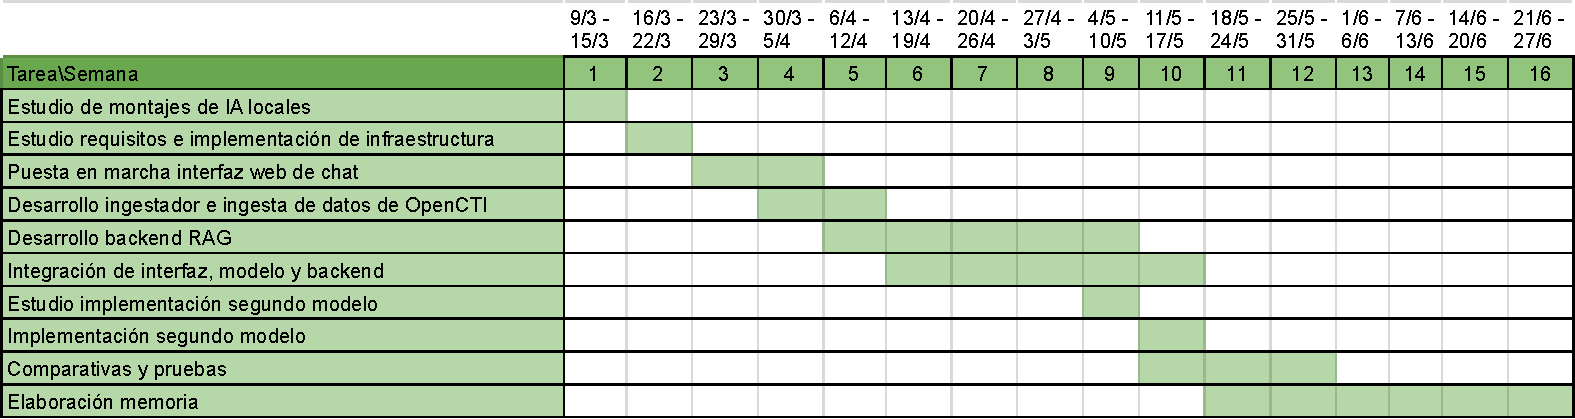
\includegraphics[width=0.95\linewidth]{Imagenes/gantt}
    \caption{Diagrama de Gantt}
    \label{fig:gantt}
\end{figure}
\begin{table}[H]
	\centering
	\begin{tabular}{l r}
		\hline
		\textbf{Tarea} & \textbf{Horas } \\
		\hline
		 Estudio de montajes de IA locales &  10 \\
		  \hline
		 Estudio requisitos e implementación de infraestructura &  10 \\
		  \hline
		 Puesta en marcha interfaz web de chat & 20  \\
		  \hline
		 Desarrollo ingestador e ingesta de datos &  25 \\
		  \hline
		 Desarrollo backend y motor RAG &  55 \\
		  \hline
		 Integración interfaz, modelo y backend & 70  \\
		  \hline
		 Estudio de segundo modelo &  5 \\
		  \hline
		 Implementación segundo modelo & 5  \\
		  \hline
		 Comparativas y pruebas &  25 \\
		  \hline
		 Desarrollo memoria &   \\
		  \hline
		 Total &  225 \\
		 \hline
	\end{tabular}
	\caption{Tabla de tareas y tiempos}
	\label{tab:tiempos}
\end{table}

\addcontentsline{toc}{subsection}{Anexo B. Ficheros desarrollados.}
\subsection*{Anexo B: Ficheros desarrollados.}
\label{sec:anexoB}

\lstinputlisting[language=Python, inputencoding=utf8/latin1, breaklines=true,caption=ingest.py,label=lst:ingest]{python/ingest.py}

\lstinputlisting[language=Python, inputencoding=utf8/latin1, breaklines=true,caption=normalizer.py,label=lst:normalizer]{python/normalizer.py}

\lstinputlisting[language=Python, inputencoding=utf8/latin1, breaklines=true,caption=normalize\_all.py,label=lst:normalizeall]{python/normalize_all.py}

\lstinputlisting[language=Python, inputencoding=utf8/latin1, breaklines=true,caption=embed\_all\_st.py,label=lst:embedall]{python/embed_all_st.py}

\lstinputlisting[language=Python, inputencoding=utf8/latin1, breaklines=true,caption=chroma\_load.py,label=lst:chromaload]{python/chroma_load.py}

\lstinputlisting[language=Python, inputencoding=utf8/latin1, breaklines=true,caption=docker-compose.yml,label=lst:dockercompose]{docker-compose.yml}

\newpage
\addcontentsline{toc}{section}{Bibliografía}
\printbibliography[title={Bibliografía}]


\end{document}